\documentclass[a4paper]{book}
\usepackage{a4wide}
\usepackage{makeidx}
\usepackage{graphicx}
\usepackage{multicol}
\usepackage{float}
\usepackage{listings}
\usepackage{color}
\usepackage{textcomp}
\usepackage{alltt}
\usepackage{times}
\usepackage{ifpdf}
\ifpdf
\usepackage[pdftex,
            pagebackref=true,
            colorlinks=true,
            linkcolor=blue,
            unicode
           ]{hyperref}
\else
\usepackage[ps2pdf,
            pagebackref=true,
            colorlinks=true,
            linkcolor=blue,
            unicode
           ]{hyperref}
\usepackage{pspicture}
\fi
\usepackage[utf8]{inputenc}
\usepackage{doxygen}
\lstset{language=C++,inputencoding=utf8,basicstyle=\footnotesize,breaklines=true,breakatwhitespace=true,tabsize=8,numbers=left }
\makeindex
\setcounter{tocdepth}{3}
\renewcommand{\footrulewidth}{0.4pt}
\begin{document}
\hypersetup{pageanchor=false}
\begin{titlepage}
\vspace*{7cm}
\begin{center}
{\Large Reference Manual}\\
\vspace*{1cm}
{\large Generated by Doxygen 1.6.1}\\
\vspace*{0.5cm}
{\small Mon Nov 16 02:24:00 2009}\\
\end{center}
\end{titlepage}
\clearemptydoublepage
\pagenumbering{roman}
\tableofcontents
\clearemptydoublepage
\pagenumbering{arabic}
\hypersetup{pageanchor=true}
\chapter{Class Index}
\section{Class Hierarchy}
This inheritance list is sorted roughly, but not completely, alphabetically:\begin{DoxyCompactList}
\item \contentsline{section}{pysusestudio::pySuseStudio}{\pageref{classpysusestudio_1_1py_suse_studio}}{}
\item \contentsline{section}{pysusestudio::pySuseStudioError}{\pageref{classpysusestudio_1_1py_suse_studio_error}}{}
\begin{DoxyCompactList}
\item \contentsline{section}{pysusestudio::APILimit}{\pageref{classpysusestudio_1_1_a_p_i_limit}}{}
\item \contentsline{section}{pysusestudio::AuthError}{\pageref{classpysusestudio_1_1_auth_error}}{}
\end{DoxyCompactList}
\end{DoxyCompactList}

\chapter{Class Index}
\section{Class List}
Here are the classes, structs, unions and interfaces with brief descriptions:\begin{DoxyCompactList}
\item\contentsline{section}{\hyperlink{classpysusestudio_1_1_a_p_i_limit}{pysusestudio::APILimit} }{\pageref{classpysusestudio_1_1_a_p_i_limit}}{}
\item\contentsline{section}{\hyperlink{classpysusestudio_1_1_auth_error}{pysusestudio::AuthError} }{\pageref{classpysusestudio_1_1_auth_error}}{}
\item\contentsline{section}{\hyperlink{classpysusestudio_1_1py_suse_studio}{pysusestudio::pySuseStudio} }{\pageref{classpysusestudio_1_1py_suse_studio}}{}
\item\contentsline{section}{\hyperlink{classpysusestudio_1_1py_suse_studio_error}{pysusestudio::pySuseStudioError} }{\pageref{classpysusestudio_1_1py_suse_studio_error}}{}
\end{DoxyCompactList}

\chapter{Class Documentation}
\hypertarget{classpysusestudio_1_1_a_p_i_limit}{
\section{pysusestudio::APILimit Class Reference}
\label{classpysusestudio_1_1_a_p_i_limit}\index{pysusestudio::APILimit@{pysusestudio::APILimit}}
}
Inheritance diagram for pysusestudio::APILimit::\begin{figure}[H]
\begin{center}
\leavevmode
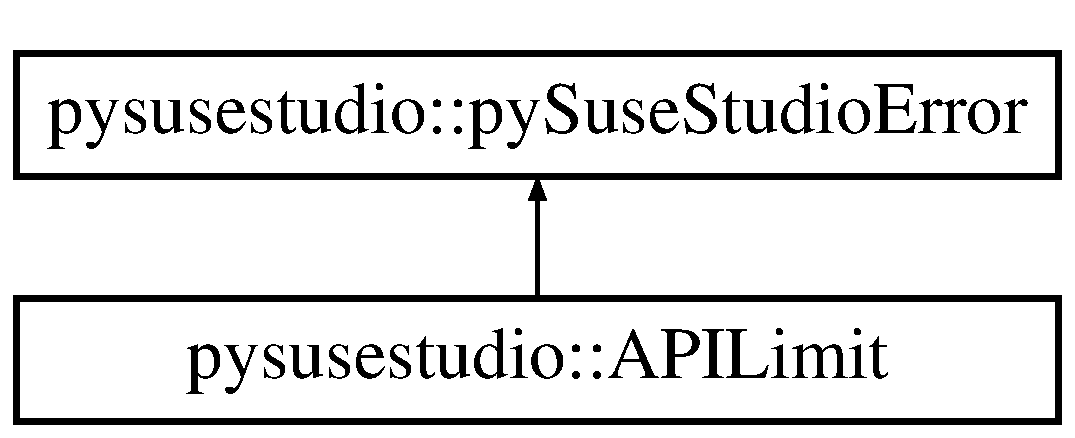
\includegraphics[height=2cm]{classpysusestudio_1_1_a_p_i_limit}
\end{center}
\end{figure}
\subsection*{Public Member Functions}
\begin{DoxyCompactItemize}
\item 
\hypertarget{classpysusestudio_1_1_a_p_i_limit_a8e376dc69f87df04e6dca8a14028bd81}{
def {\bfseries \_\-\_\-init\_\-\_\-}}
\label{classpysusestudio_1_1_a_p_i_limit_a8e376dc69f87df04e6dca8a14028bd81}

\item 
\hypertarget{classpysusestudio_1_1_a_p_i_limit_ad0a553cc2380422beaeb1a1c2b000855}{
def {\bfseries \_\-\_\-str\_\-\_\-}}
\label{classpysusestudio_1_1_a_p_i_limit_ad0a553cc2380422beaeb1a1c2b000855}

\end{DoxyCompactItemize}
\subsection*{Public Attributes}
\begin{DoxyCompactItemize}
\item 
\hypertarget{classpysusestudio_1_1_a_p_i_limit_a96d8ae9a2eb1e786576b72c59079410b}{
{\bfseries msg}}
\label{classpysusestudio_1_1_a_p_i_limit_a96d8ae9a2eb1e786576b72c59079410b}

\end{DoxyCompactItemize}


The documentation for this class was generated from the following file:\begin{DoxyCompactItemize}
\item 
pysusestudio.py\end{DoxyCompactItemize}

\hypertarget{classpysusestudio_1_1_auth_error}{
\section{pysusestudio::AuthError Class Reference}
\label{classpysusestudio_1_1_auth_error}\index{pysusestudio::AuthError@{pysusestudio::AuthError}}
}
Inheritance diagram for pysusestudio::AuthError::\begin{figure}[H]
\begin{center}
\leavevmode
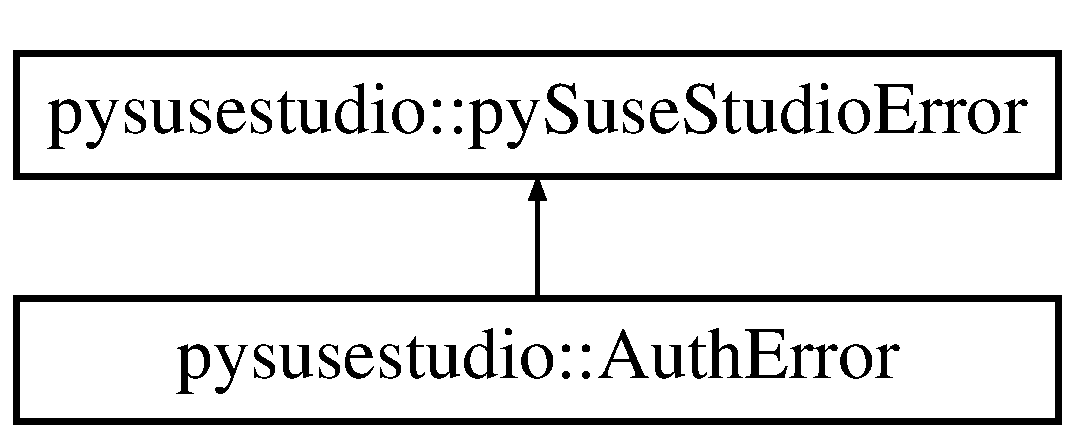
\includegraphics[height=2cm]{classpysusestudio_1_1_auth_error}
\end{center}
\end{figure}
\subsection*{Public Member Functions}
\begin{DoxyCompactItemize}
\item 
\hypertarget{classpysusestudio_1_1_auth_error_a71690316a4d97777e77e484d31183509}{
def {\bfseries \_\-\_\-init\_\-\_\-}}
\label{classpysusestudio_1_1_auth_error_a71690316a4d97777e77e484d31183509}

\item 
\hypertarget{classpysusestudio_1_1_auth_error_ae3d558da4555fc4285185b9f1afcad18}{
def {\bfseries \_\-\_\-str\_\-\_\-}}
\label{classpysusestudio_1_1_auth_error_ae3d558da4555fc4285185b9f1afcad18}

\end{DoxyCompactItemize}
\subsection*{Public Attributes}
\begin{DoxyCompactItemize}
\item 
\hypertarget{classpysusestudio_1_1_auth_error_a32ce5c08c2034b562f1d99aaa1166cf2}{
{\bfseries msg}}
\label{classpysusestudio_1_1_auth_error_a32ce5c08c2034b562f1d99aaa1166cf2}

\end{DoxyCompactItemize}


The documentation for this class was generated from the following file:\begin{DoxyCompactItemize}
\item 
pysusestudio.py\end{DoxyCompactItemize}

\hypertarget{classpysusestudio_1_1py_suse_studio}{
\section{pysusestudio::pySuseStudio Class Reference}
\label{classpysusestudio_1_1py_suse_studio}\index{pysusestudio::pySuseStudio@{pysusestudio::pySuseStudio}}
}
\subsection*{Public Member Functions}
\begin{DoxyCompactItemize}
\item 
def \hyperlink{classpysusestudio_1_1py_suse_studio_a8067ee791da6de5d42fa2954d6eff0ce}{\_\-\_\-init\_\-\_\-}
\item 
\hypertarget{classpysusestudio_1_1py_suse_studio_a69265b9890834789bfc75b8d8dbe1738}{
def {\bfseries buildApiURL}}
\label{classpysusestudio_1_1py_suse_studio_a69265b9890834789bfc75b8d8dbe1738}

\item 
def \hyperlink{classpysusestudio_1_1py_suse_studio_a1b0687dee747d4237b2a4e979d6cbe3a}{getAccount}
\item 
def \hyperlink{classpysusestudio_1_1py_suse_studio_ada8fe51f723f7ccf7c7f2fe618281150}{getApiKey}
\item 
def \hyperlink{classpysusestudio_1_1py_suse_studio_acfcc75e5a423bc1579431ed9e0e56997}{getTemplateSets}
\item 
def \hyperlink{classpysusestudio_1_1py_suse_studio_afc468bc6f14f91cc718159d0118562f9}{getAppliances}
\item 
def \hyperlink{classpysusestudio_1_1py_suse_studio_a0e4301835de3e52a600c536d5a6a22d6}{setAppliances}
\item 
def \hyperlink{classpysusestudio_1_1py_suse_studio_a6f83ab270f1292009bc396fd51cee83f}{delAppliances}
\item 
def \hyperlink{classpysusestudio_1_1py_suse_studio_aa9ac2b217553d0e92c065a023ecb159b}{getRepositories}
\item 
def \hyperlink{classpysusestudio_1_1py_suse_studio_af52249bbd81c55a5a1d4253ac28c9647}{putRepositories}
\item 
def \hyperlink{classpysusestudio_1_1py_suse_studio_a9ae92820c58858bf901366c3d003b305}{setRepositories}
\item 
def \hyperlink{classpysusestudio_1_1py_suse_studio_a25daf579acd05aa6b674fa2e7c61e2f8}{delRepositories}
\item 
def \hyperlink{classpysusestudio_1_1py_suse_studio_a310e27602fda6a8c78bbc583ab882d76}{addRepositoryUser}
\item 
def \hyperlink{classpysusestudio_1_1py_suse_studio_a629c7120bc2bb4bcbb3f5bd687b7a81b}{getSoftware}
\item 
def \hyperlink{classpysusestudio_1_1py_suse_studio_ab776945c6d116ac2d2e8acdace99e623}{putSoftware}
\item 
def \hyperlink{classpysusestudio_1_1py_suse_studio_a9ee9e20b9c942e502c1d45552d118c18}{getSoftwareInstalled}
\item 
def \hyperlink{classpysusestudio_1_1py_suse_studio_aff587b16668414a1f2e393bf0aab6943}{addSoftwarePackage}
\item 
def \hyperlink{classpysusestudio_1_1py_suse_studio_a85fb426704d174487ce90469476e319a}{delSoftwarePackage}
\item 
def \hyperlink{classpysusestudio_1_1py_suse_studio_ab6ed7add2eb09cde2c9b85c9b40c7e3a}{addSoftwarePattern}
\item 
def \hyperlink{classpysusestudio_1_1py_suse_studio_a05a10bd3b9fdf4eac43d620a9dde588f}{delSoftwarePattern}
\item 
def \hyperlink{classpysusestudio_1_1py_suse_studio_ad74a578d8eee03662b2a157a98798dbd}{searchSoftware}
\item 
def \hyperlink{classpysusestudio_1_1py_suse_studio_a9af6672216c4ce9c3684433b83b19a8e}{getOverlayFiles}
\item 
def \hyperlink{classpysusestudio_1_1py_suse_studio_a37506f6f8cd8fc081a8f40bbdacf1de5}{addOverlayFiles}
\item 
def \hyperlink{classpysusestudio_1_1py_suse_studio_a9afaf308e7145e0ece5f6ef04385c537}{getOverlayFile}
\item 
def \hyperlink{classpysusestudio_1_1py_suse_studio_a18433f6c2be7dd749e2d7999e28b14f6}{getOverlayFileMeta}
\item 
def \hyperlink{classpysusestudio_1_1py_suse_studio_aabf405f8c1c7b56b71a2d4911a3df813}{putOverlayFile}
\item 
def \hyperlink{classpysusestudio_1_1py_suse_studio_a0190fc73980adef1a17b4d096012a35c}{putOverlayFileMeta}
\item 
def \hyperlink{classpysusestudio_1_1py_suse_studio_a4709eddea40e484a40f499e07c67f698}{delOverlayFile}
\item 
def \hyperlink{classpysusestudio_1_1py_suse_studio_a605349d59cf89acb5aabe7b810c9de41}{getRunningBuilds}
\item 
def \hyperlink{classpysusestudio_1_1py_suse_studio_a1b5b2d3eb030841b1d50117cb081d935}{getRunningBuild}
\item 
def \hyperlink{classpysusestudio_1_1py_suse_studio_adf21425727a0efca0a8bd8aab4126ce0}{addBuild}
\item 
def \hyperlink{classpysusestudio_1_1py_suse_studio_a00a994e839162b466150f65b96c79d53}{delRunningBuild}
\item 
def \hyperlink{classpysusestudio_1_1py_suse_studio_a2dce0b6f9b748795beadf6b7776f2ebf}{getCompletedBuilds}
\item 
def \hyperlink{classpysusestudio_1_1py_suse_studio_afea5cfcc56e614dfc6b78f8d79f8ac4d}{getCompletedBuild}
\item 
def \hyperlink{classpysusestudio_1_1py_suse_studio_af4e1c32a537d923d174dd3dce2af889b}{delCompletedBuild}
\item 
def \hyperlink{classpysusestudio_1_1py_suse_studio_a976d655984cc08a73ab2a37192012d34}{getRPMs}
\item 
def \hyperlink{classpysusestudio_1_1py_suse_studio_a351aea7ec7f00979680d2a9a1ad116bc}{getRPMInfo}
\item 
def \hyperlink{classpysusestudio_1_1py_suse_studio_a57ade7463c2ed61ba29b096f7a084b44}{getRPM}
\item 
def \hyperlink{classpysusestudio_1_1py_suse_studio_aa0a1478f603ec4913db98d7de866e7f7}{addRPM}
\item 
def \hyperlink{classpysusestudio_1_1py_suse_studio_a5d0e4733f7efe9d879110b44848cc4da}{putRPM}
\item 
def \hyperlink{classpysusestudio_1_1py_suse_studio_a91d190ecb9f6590fbc9268724a65b87d}{delRPM}
\item 
def \hyperlink{classpysusestudio_1_1py_suse_studio_aa9ac2b217553d0e92c065a023ecb159b}{getRepositories}
\item 
def \hyperlink{classpysusestudio_1_1py_suse_studio_a226b08a0195091512cd73c33881aa3ac}{getRepository}
\item 
def \hyperlink{classpysusestudio_1_1py_suse_studio_a19fd7008b36708fad6cbb4a06df68bdb}{addRepository}
\item 
def \hyperlink{classpysusestudio_1_1py_suse_studio_a0c239e92b36b5de984effab04f51417a}{version}
\end{DoxyCompactItemize}
\subsection*{Public Attributes}
\begin{DoxyCompactItemize}
\item 
\hypertarget{classpysusestudio_1_1py_suse_studio_a6b9cb8b7ed1ce7ed73fd597cf9dde1fb}{
{\bfseries authenticated}}
\label{classpysusestudio_1_1py_suse_studio_a6b9cb8b7ed1ce7ed73fd597cf9dde1fb}

\item 
\hypertarget{classpysusestudio_1_1py_suse_studio_a055a7f27f63a9eada50b8eba479ba2cf}{
{\bfseries username}}
\label{classpysusestudio_1_1py_suse_studio_a055a7f27f63a9eada50b8eba479ba2cf}

\item 
\hypertarget{classpysusestudio_1_1py_suse_studio_a70a18473f5f26843fde2690d897dfaf2}{
{\bfseries password}}
\label{classpysusestudio_1_1py_suse_studio_a70a18473f5f26843fde2690d897dfaf2}

\item 
\hypertarget{classpysusestudio_1_1py_suse_studio_af2712d0574ce6b87e2dfc2530850a1ee}{
{\bfseries address}}
\label{classpysusestudio_1_1py_suse_studio_af2712d0574ce6b87e2dfc2530850a1ee}

\item 
\hypertarget{classpysusestudio_1_1py_suse_studio_aa77c8b7fb2fb777c9d7e436ffbb0ae7e}{
{\bfseries auth\_\-manager}}
\label{classpysusestudio_1_1py_suse_studio_aa77c8b7fb2fb777c9d7e436ffbb0ae7e}

\item 
\hypertarget{classpysusestudio_1_1py_suse_studio_aa8b0221e970433ec3be8f812e90d6ebe}{
{\bfseries handler}}
\label{classpysusestudio_1_1py_suse_studio_aa8b0221e970433ec3be8f812e90d6ebe}

\item 
\hypertarget{classpysusestudio_1_1py_suse_studio_a05bc44a7df4c292fbe044c05db8d646c}{
{\bfseries opener}}
\label{classpysusestudio_1_1py_suse_studio_a05bc44a7df4c292fbe044c05db8d646c}

\end{DoxyCompactItemize}


\subsection{Member Function Documentation}
\hypertarget{classpysusestudio_1_1py_suse_studio_a8067ee791da6de5d42fa2954d6eff0ce}{
\index{pysusestudio::pySuseStudio@{pysusestudio::pySuseStudio}!\_\-\_\-init\_\-\_\-@{\_\-\_\-init\_\-\_\-}}
\index{\_\-\_\-init\_\-\_\-@{\_\-\_\-init\_\-\_\-}!pysusestudio::pySuseStudio@{pysusestudio::pySuseStudio}}
\subsubsection[{\_\-\_\-init\_\-\_\-}]{\setlength{\rightskip}{0pt plus 5cm}def pysusestudio::pySuseStudio::\_\-\_\-init\_\-\_\- ( {\em self}, \/   {\em username} = {\ttfamily None}, \/   {\em password} = {\ttfamily None}, \/   {\em headers} = {\ttfamily None})}}
\label{classpysusestudio_1_1py_suse_studio_a8067ee791da6de5d42fa2954d6eff0ce}
\begin{DoxyVerb}pySuseStudio( username = None, password = None, headers = None)

        Instantiates an instance of pySuseStudio. Takes optional parameters for authentication and such (see below).

        Parameters:
username - Your Suse Studio username, if you want Basic (HTTP) Authentication.
password - Your Suse Studio secret key, if you want Basic (HTTP) Authentication.
headers - User agent header.
\end{DoxyVerb}
 \hypertarget{classpysusestudio_1_1py_suse_studio_adf21425727a0efca0a8bd8aab4126ce0}{
\index{pysusestudio::pySuseStudio@{pysusestudio::pySuseStudio}!addBuild@{addBuild}}
\index{addBuild@{addBuild}!pysusestudio::pySuseStudio@{pysusestudio::pySuseStudio}}
\subsubsection[{addBuild}]{\setlength{\rightskip}{0pt plus 5cm}def pysusestudio::pySuseStudio::addBuild ( {\em self}, \/   {\em id}, \/   {\em force} = {\ttfamily None}, \/   {\em version} = {\ttfamily None}, \/   {\em image\_\-type} = {\ttfamily None})}}
\label{classpysusestudio_1_1py_suse_studio_adf21425727a0efca0a8bd8aab4126ce0}
\begin{DoxyVerb}addBuild(id, force=None, version=None, image_type=None)

            Start a new build for the given id appliance. 
            If there already is a build with the same appliance settings (build type and version) 
            an error is returned. In this case a build can be enforced by setting the optional 
            force parameter to true.
            Optionally the appliance version and build type can be set with the version and image_type parameters. 
            
            Parameters:
id - Id of the appliance
force (optional) - Force a build even if it overwrites an already existing build. 
version (optional) - The version of the appliance. 
image_type (optional) -  The format of the build. Supported are 'xen','oem','vmx' and 'iso'. 

\end{DoxyVerb}
 \hypertarget{classpysusestudio_1_1py_suse_studio_a37506f6f8cd8fc081a8f40bbdacf1de5}{
\index{pysusestudio::pySuseStudio@{pysusestudio::pySuseStudio}!addOverlayFiles@{addOverlayFiles}}
\index{addOverlayFiles@{addOverlayFiles}!pysusestudio::pySuseStudio@{pysusestudio::pySuseStudio}}
\subsubsection[{addOverlayFiles}]{\setlength{\rightskip}{0pt plus 5cm}def pysusestudio::pySuseStudio::addOverlayFiles ( {\em self}, \/   {\em id}, \/   {\em body}, \/   {\em filename} = {\ttfamily None}, \/   {\em path} = {\ttfamily None}, \/   {\em owner} = {\ttfamily None}, \/   {\em group} = {\ttfamily None}, \/   {\em permissions} = {\ttfamily None}, \/   {\em enabled} = {\ttfamily None})}}
\label{classpysusestudio_1_1py_suse_studio_a37506f6f8cd8fc081a8f40bbdacf1de5}
\begin{DoxyVerb}addOverlayFiles(id, body, filename=None, path=None, owner=None, group=None, permissions=None, enabled=None)

            Adds a file to the given id appliance. 
            Optionally, one or more metadata settings can be specified. If those are left out, they 
            can also be change later. 
            
            Parameters:
id - Id of the appliance
body - the entity body to be sent with the request.
filename (optional) - The name of the file in the filesystem. 
path (optional) - The path where the file will be stored. 
owner (optional) - The owner of the file. 
group (optional) - The group of the file. 
permissions (optional) - The permissions of the file. 
enabled (optional) - Used to enable/disable this file for the builds. 

\end{DoxyVerb}
 \hypertarget{classpysusestudio_1_1py_suse_studio_a19fd7008b36708fad6cbb4a06df68bdb}{
\index{pysusestudio::pySuseStudio@{pysusestudio::pySuseStudio}!addRepository@{addRepository}}
\index{addRepository@{addRepository}!pysusestudio::pySuseStudio@{pysusestudio::pySuseStudio}}
\subsubsection[{addRepository}]{\setlength{\rightskip}{0pt plus 5cm}def pysusestudio::pySuseStudio::addRepository ( {\em self}, \/   {\em repo\_\-url}, \/   {\em name})}}
\label{classpysusestudio_1_1py_suse_studio_a19fd7008b36708fad6cbb4a06df68bdb}
\begin{DoxyVerb}addRepository(repo_url, name)

            Imports a new repository into Studio. Returns the metadata for the created repository
            
            Parameters:
repo_url - Base url of the repository. 
name - Name for the repository. 

\end{DoxyVerb}
 \hypertarget{classpysusestudio_1_1py_suse_studio_a310e27602fda6a8c78bbc583ab882d76}{
\index{pysusestudio::pySuseStudio@{pysusestudio::pySuseStudio}!addRepositoryUser@{addRepositoryUser}}
\index{addRepositoryUser@{addRepositoryUser}!pysusestudio::pySuseStudio@{pysusestudio::pySuseStudio}}
\subsubsection[{addRepositoryUser}]{\setlength{\rightskip}{0pt plus 5cm}def pysusestudio::pySuseStudio::addRepositoryUser ( {\em self}, \/   {\em id})}}
\label{classpysusestudio_1_1py_suse_studio_a310e27602fda6a8c78bbc583ab882d76}
\begin{DoxyVerb}addRepositoryUser(id)

            Adds the according user repository (the one containing the uploaded RPMs) to the appliance
            
            Parameters:
id - Id of the appliance

\end{DoxyVerb}
 \hypertarget{classpysusestudio_1_1py_suse_studio_aa0a1478f603ec4913db98d7de866e7f7}{
\index{pysusestudio::pySuseStudio@{pysusestudio::pySuseStudio}!addRPM@{addRPM}}
\index{addRPM@{addRPM}!pysusestudio::pySuseStudio@{pysusestudio::pySuseStudio}}
\subsubsection[{addRPM}]{\setlength{\rightskip}{0pt plus 5cm}def pysusestudio::pySuseStudio::addRPM ( {\em self}, \/   {\em base})}}
\label{classpysusestudio_1_1py_suse_studio_aa0a1478f603ec4913db98d7de866e7f7}
\begin{DoxyVerb}addBuild(base)

            Adds an RPM or archive to the user repository for appliances base 
            
            Parameters:
base - Base system of the RPM or archive, e.g. 11.1 or SLED11.


\end{DoxyVerb}
 \hypertarget{classpysusestudio_1_1py_suse_studio_aff587b16668414a1f2e393bf0aab6943}{
\index{pysusestudio::pySuseStudio@{pysusestudio::pySuseStudio}!addSoftwarePackage@{addSoftwarePackage}}
\index{addSoftwarePackage@{addSoftwarePackage}!pysusestudio::pySuseStudio@{pysusestudio::pySuseStudio}}
\subsubsection[{addSoftwarePackage}]{\setlength{\rightskip}{0pt plus 5cm}def pysusestudio::pySuseStudio::addSoftwarePackage ( {\em self}, \/   {\em id}, \/   {\em name}, \/   {\em version} = {\ttfamily None}, \/   {\em repository\_\-id} = {\ttfamily None})}}
\label{classpysusestudio_1_1py_suse_studio_aff587b16668414a1f2e393bf0aab6943}
\begin{DoxyVerb}addSoftwarePackage(id, name, version=None, repository_id=None)

            Add specified package to the given appliance
            
            Parameters:
id - Id of the appliance
name - Name of the package
version (optional) - Version of the package
repository_id (optional) - Repository to pick the package from

\end{DoxyVerb}
 \hypertarget{classpysusestudio_1_1py_suse_studio_ab6ed7add2eb09cde2c9b85c9b40c7e3a}{
\index{pysusestudio::pySuseStudio@{pysusestudio::pySuseStudio}!addSoftwarePattern@{addSoftwarePattern}}
\index{addSoftwarePattern@{addSoftwarePattern}!pysusestudio::pySuseStudio@{pysusestudio::pySuseStudio}}
\subsubsection[{addSoftwarePattern}]{\setlength{\rightskip}{0pt plus 5cm}def pysusestudio::pySuseStudio::addSoftwarePattern ( {\em self}, \/   {\em id}, \/   {\em name}, \/   {\em version} = {\ttfamily None}, \/   {\em repository\_\-id} = {\ttfamily None})}}
\label{classpysusestudio_1_1py_suse_studio_ab6ed7add2eb09cde2c9b85c9b40c7e3a}
\begin{DoxyVerb}addSoftwarePattern(id, name, version=None, repository_id=None)

            Add specified pattern to the given appliance
            
            Parameters:
id - Id of the appliance
name - Name of the pattern
version (optional) - Version of the pattern
repository_id (optional) - Repository to pick the pattern from

\end{DoxyVerb}
 \hypertarget{classpysusestudio_1_1py_suse_studio_a6f83ab270f1292009bc396fd51cee83f}{
\index{pysusestudio::pySuseStudio@{pysusestudio::pySuseStudio}!delAppliances@{delAppliances}}
\index{delAppliances@{delAppliances}!pysusestudio::pySuseStudio@{pysusestudio::pySuseStudio}}
\subsubsection[{delAppliances}]{\setlength{\rightskip}{0pt plus 5cm}def pysusestudio::pySuseStudio::delAppliances ( {\em self}, \/   {\em id})}}
\label{classpysusestudio_1_1py_suse_studio_a6f83ab270f1292009bc396fd51cee83f}
\begin{DoxyVerb}delAppliances(self, id)

        Delete appliance with given id. 
            
            Parameters:
id - Id of the appliance

\end{DoxyVerb}
 \hypertarget{classpysusestudio_1_1py_suse_studio_af4e1c32a537d923d174dd3dce2af889b}{
\index{pysusestudio::pySuseStudio@{pysusestudio::pySuseStudio}!delCompletedBuild@{delCompletedBuild}}
\index{delCompletedBuild@{delCompletedBuild}!pysusestudio::pySuseStudio@{pysusestudio::pySuseStudio}}
\subsubsection[{delCompletedBuild}]{\setlength{\rightskip}{0pt plus 5cm}def pysusestudio::pySuseStudio::delCompletedBuild ( {\em self}, \/   {\em id})}}
\label{classpysusestudio_1_1py_suse_studio_af4e1c32a537d923d174dd3dce2af889b}
\begin{DoxyVerb}delCompletedBuild(id)

            Delete specified completed build
            
            Parameters:
id - Id of the running build

\end{DoxyVerb}
 \hypertarget{classpysusestudio_1_1py_suse_studio_a4709eddea40e484a40f499e07c67f698}{
\index{pysusestudio::pySuseStudio@{pysusestudio::pySuseStudio}!delOverlayFile@{delOverlayFile}}
\index{delOverlayFile@{delOverlayFile}!pysusestudio::pySuseStudio@{pysusestudio::pySuseStudio}}
\subsubsection[{delOverlayFile}]{\setlength{\rightskip}{0pt plus 5cm}def pysusestudio::pySuseStudio::delOverlayFile ( {\em self}, \/   {\em id})}}
\label{classpysusestudio_1_1py_suse_studio_a4709eddea40e484a40f499e07c67f698}
\begin{DoxyVerb}delOverlayFile(id)

            Delete specified overlay file
            
            Parameters:
id - Id of the file

\end{DoxyVerb}
 \hypertarget{classpysusestudio_1_1py_suse_studio_a25daf579acd05aa6b674fa2e7c61e2f8}{
\index{pysusestudio::pySuseStudio@{pysusestudio::pySuseStudio}!delRepositories@{delRepositories}}
\index{delRepositories@{delRepositories}!pysusestudio::pySuseStudio@{pysusestudio::pySuseStudio}}
\subsubsection[{delRepositories}]{\setlength{\rightskip}{0pt plus 5cm}def pysusestudio::pySuseStudio::delRepositories ( {\em self}, \/   {\em id}, \/   {\em repo\_\-id})}}
\label{classpysusestudio_1_1py_suse_studio_a25daf579acd05aa6b674fa2e7c61e2f8}
\begin{DoxyVerb}delRepositories(id, repo_id)

            Remove the specified repository to the given id appliance
            
            Parameters:
id - Id of the appliance
repo_id - Id of the repository

\end{DoxyVerb}
 \hypertarget{classpysusestudio_1_1py_suse_studio_a91d190ecb9f6590fbc9268724a65b87d}{
\index{pysusestudio::pySuseStudio@{pysusestudio::pySuseStudio}!delRPM@{delRPM}}
\index{delRPM@{delRPM}!pysusestudio::pySuseStudio@{pysusestudio::pySuseStudio}}
\subsubsection[{delRPM}]{\setlength{\rightskip}{0pt plus 5cm}def pysusestudio::pySuseStudio::delRPM ( {\em self}, \/   {\em id})}}
\label{classpysusestudio_1_1py_suse_studio_a91d190ecb9f6590fbc9268724a65b87d}
\begin{DoxyVerb}delRPM(id)

            Deletes the RPM or archive with the given id from the user repository
            
            Parameters:
id - id of the uploaded RPM.

\end{DoxyVerb}
 \hypertarget{classpysusestudio_1_1py_suse_studio_a00a994e839162b466150f65b96c79d53}{
\index{pysusestudio::pySuseStudio@{pysusestudio::pySuseStudio}!delRunningBuild@{delRunningBuild}}
\index{delRunningBuild@{delRunningBuild}!pysusestudio::pySuseStudio@{pysusestudio::pySuseStudio}}
\subsubsection[{delRunningBuild}]{\setlength{\rightskip}{0pt plus 5cm}def pysusestudio::pySuseStudio::delRunningBuild ( {\em self}, \/   {\em id})}}
\label{classpysusestudio_1_1py_suse_studio_a00a994e839162b466150f65b96c79d53}
\begin{DoxyVerb}delRunningBuild(id)

            Delete specified running build
            
            Parameters:
id - Id of the running build

\end{DoxyVerb}
 \hypertarget{classpysusestudio_1_1py_suse_studio_a85fb426704d174487ce90469476e319a}{
\index{pysusestudio::pySuseStudio@{pysusestudio::pySuseStudio}!delSoftwarePackage@{delSoftwarePackage}}
\index{delSoftwarePackage@{delSoftwarePackage}!pysusestudio::pySuseStudio@{pysusestudio::pySuseStudio}}
\subsubsection[{delSoftwarePackage}]{\setlength{\rightskip}{0pt plus 5cm}def pysusestudio::pySuseStudio::delSoftwarePackage ( {\em self}, \/   {\em id}, \/   {\em name})}}
\label{classpysusestudio_1_1py_suse_studio_a85fb426704d174487ce90469476e319a}
\begin{DoxyVerb}delSoftwarePackage(id, name)

            Delete specified package from the given appliance
            
            Parameters:
id - Id of the appliance
name - Name of the package

\end{DoxyVerb}
 \hypertarget{classpysusestudio_1_1py_suse_studio_a05a10bd3b9fdf4eac43d620a9dde588f}{
\index{pysusestudio::pySuseStudio@{pysusestudio::pySuseStudio}!delSoftwarePattern@{delSoftwarePattern}}
\index{delSoftwarePattern@{delSoftwarePattern}!pysusestudio::pySuseStudio@{pysusestudio::pySuseStudio}}
\subsubsection[{delSoftwarePattern}]{\setlength{\rightskip}{0pt plus 5cm}def pysusestudio::pySuseStudio::delSoftwarePattern ( {\em self}, \/   {\em id}, \/   {\em name})}}
\label{classpysusestudio_1_1py_suse_studio_a05a10bd3b9fdf4eac43d620a9dde588f}
\begin{DoxyVerb}delSoftwarePattern(id, name)

            Delete specified pattern from the given appliance
            
            Parameters:
id - Id of the appliance
name - Name of the pattern

\end{DoxyVerb}
 \hypertarget{classpysusestudio_1_1py_suse_studio_a1b0687dee747d4237b2a4e979d6cbe3a}{
\index{pysusestudio::pySuseStudio@{pysusestudio::pySuseStudio}!getAccount@{getAccount}}
\index{getAccount@{getAccount}!pysusestudio::pySuseStudio@{pysusestudio::pySuseStudio}}
\subsubsection[{getAccount}]{\setlength{\rightskip}{0pt plus 5cm}def pysusestudio::pySuseStudio::getAccount ( {\em self})}}
\label{classpysusestudio_1_1py_suse_studio_a1b0687dee747d4237b2a4e979d6cbe3a}
\begin{DoxyVerb}getAccount()

        Returns information about the account, such as username, email address and disk quota.
\end{DoxyVerb}
 \hypertarget{classpysusestudio_1_1py_suse_studio_ada8fe51f723f7ccf7c7f2fe618281150}{
\index{pysusestudio::pySuseStudio@{pysusestudio::pySuseStudio}!getApiKey@{getApiKey}}
\index{getApiKey@{getApiKey}!pysusestudio::pySuseStudio@{pysusestudio::pySuseStudio}}
\subsubsection[{getApiKey}]{\setlength{\rightskip}{0pt plus 5cm}def pysusestudio::pySuseStudio::getApiKey ( {\em self})}}
\label{classpysusestudio_1_1py_suse_studio_ada8fe51f723f7ccf7c7f2fe618281150}
\begin{DoxyVerb}getApiKey()

        Returns an HTML page which contains the API key flagged as:

            <span class="studio:api_key">ksdjfu93r</span>. 
            
\end{DoxyVerb}
 \hypertarget{classpysusestudio_1_1py_suse_studio_afc468bc6f14f91cc718159d0118562f9}{
\index{pysusestudio::pySuseStudio@{pysusestudio::pySuseStudio}!getAppliances@{getAppliances}}
\index{getAppliances@{getAppliances}!pysusestudio::pySuseStudio@{pysusestudio::pySuseStudio}}
\subsubsection[{getAppliances}]{\setlength{\rightskip}{0pt plus 5cm}def pysusestudio::pySuseStudio::getAppliances ( {\em self}, \/   {\em id} = {\ttfamily None}, \/   {\em status} = {\ttfamily False})}}
\label{classpysusestudio_1_1py_suse_studio_afc468bc6f14f91cc718159d0118562f9}
\begin{DoxyVerb}getAppliances(id = None, status = False)

        List all appliances of the current user.  
            
            Parameters:
id - Optional. Id of the appliance
status - Optional. If true get status of given Id appliance

\end{DoxyVerb}
 \hypertarget{classpysusestudio_1_1py_suse_studio_afea5cfcc56e614dfc6b78f8d79f8ac4d}{
\index{pysusestudio::pySuseStudio@{pysusestudio::pySuseStudio}!getCompletedBuild@{getCompletedBuild}}
\index{getCompletedBuild@{getCompletedBuild}!pysusestudio::pySuseStudio@{pysusestudio::pySuseStudio}}
\subsubsection[{getCompletedBuild}]{\setlength{\rightskip}{0pt plus 5cm}def pysusestudio::pySuseStudio::getCompletedBuild ( {\em self}, \/   {\em id})}}
\label{classpysusestudio_1_1py_suse_studio_afea5cfcc56e614dfc6b78f8d79f8ac4d}
\begin{DoxyVerb}getCompletedBuild(id)

       Show build info of the build with the given id .
        
            Parameters:
id - Id of the build

\end{DoxyVerb}
 \hypertarget{classpysusestudio_1_1py_suse_studio_a2dce0b6f9b748795beadf6b7776f2ebf}{
\index{pysusestudio::pySuseStudio@{pysusestudio::pySuseStudio}!getCompletedBuilds@{getCompletedBuilds}}
\index{getCompletedBuilds@{getCompletedBuilds}!pysusestudio::pySuseStudio@{pysusestudio::pySuseStudio}}
\subsubsection[{getCompletedBuilds}]{\setlength{\rightskip}{0pt plus 5cm}def pysusestudio::pySuseStudio::getCompletedBuilds ( {\em self}, \/   {\em id})}}
\label{classpysusestudio_1_1py_suse_studio_a2dce0b6f9b748795beadf6b7776f2ebf}
\begin{DoxyVerb}getCompletedBuilds(id)

        List all completed builds for the appliance with the given id .
        
            Parameters:
id - Id of the appliance

\end{DoxyVerb}
 \hypertarget{classpysusestudio_1_1py_suse_studio_a9afaf308e7145e0ece5f6ef04385c537}{
\index{pysusestudio::pySuseStudio@{pysusestudio::pySuseStudio}!getOverlayFile@{getOverlayFile}}
\index{getOverlayFile@{getOverlayFile}!pysusestudio::pySuseStudio@{pysusestudio::pySuseStudio}}
\subsubsection[{getOverlayFile}]{\setlength{\rightskip}{0pt plus 5cm}def pysusestudio::pySuseStudio::getOverlayFile ( {\em self}, \/   {\em id})}}
\label{classpysusestudio_1_1py_suse_studio_a9afaf308e7145e0ece5f6ef04385c537}
\begin{DoxyVerb}getOverlayFile(id)

        Return overlay file with the given id .
        
            Parameters:
id - Id of the file

\end{DoxyVerb}
 \hypertarget{classpysusestudio_1_1py_suse_studio_a18433f6c2be7dd749e2d7999e28b14f6}{
\index{pysusestudio::pySuseStudio@{pysusestudio::pySuseStudio}!getOverlayFileMeta@{getOverlayFileMeta}}
\index{getOverlayFileMeta@{getOverlayFileMeta}!pysusestudio::pySuseStudio@{pysusestudio::pySuseStudio}}
\subsubsection[{getOverlayFileMeta}]{\setlength{\rightskip}{0pt plus 5cm}def pysusestudio::pySuseStudio::getOverlayFileMeta ( {\em self}, \/   {\em id})}}
\label{classpysusestudio_1_1py_suse_studio_a18433f6c2be7dd749e2d7999e28b14f6}
\begin{DoxyVerb}getOverlayFileMeta(id)

        Return overlay file meta data with the given id .
        
            Parameters:
id - Id of the file

\end{DoxyVerb}
 \hypertarget{classpysusestudio_1_1py_suse_studio_a9af6672216c4ce9c3684433b83b19a8e}{
\index{pysusestudio::pySuseStudio@{pysusestudio::pySuseStudio}!getOverlayFiles@{getOverlayFiles}}
\index{getOverlayFiles@{getOverlayFiles}!pysusestudio::pySuseStudio@{pysusestudio::pySuseStudio}}
\subsubsection[{getOverlayFiles}]{\setlength{\rightskip}{0pt plus 5cm}def pysusestudio::pySuseStudio::getOverlayFiles ( {\em self}, \/   {\em id})}}
\label{classpysusestudio_1_1py_suse_studio_a9af6672216c4ce9c3684433b83b19a8e}
\begin{DoxyVerb}getOverlayFiles(id)

        List all overlay files of the given id appliance.
        
            Parameters:
id - Id of the appliance

\end{DoxyVerb}
 \hypertarget{classpysusestudio_1_1py_suse_studio_aa9ac2b217553d0e92c065a023ecb159b}{
\index{pysusestudio::pySuseStudio@{pysusestudio::pySuseStudio}!getRepositories@{getRepositories}}
\index{getRepositories@{getRepositories}!pysusestudio::pySuseStudio@{pysusestudio::pySuseStudio}}
\subsubsection[{getRepositories}]{\setlength{\rightskip}{0pt plus 5cm}def pysusestudio::pySuseStudio::getRepositories ( {\em self}, \/   {\em base} = {\ttfamily None}, \/   {\em filter} = {\ttfamily None})}}
\label{classpysusestudio_1_1py_suse_studio_aa9ac2b217553d0e92c065a023ecb159b}
\begin{DoxyVerb}getRepositories(base=None, filter=None)

        Returns a list of repositories. If neither base system nor filter are specified all available repositories 
        are returned. 
        When filtering the results with the filter parameter, the repository name, repository url and repository 
        packages are searched.
        
            Parameters:
base (optional) - Limit the results to repositories with this base system. 
filter (optional) - Only show repositories matching this search string.

\end{DoxyVerb}
 \hypertarget{classpysusestudio_1_1py_suse_studio_aa9ac2b217553d0e92c065a023ecb159b}{
\index{pysusestudio::pySuseStudio@{pysusestudio::pySuseStudio}!getRepositories@{getRepositories}}
\index{getRepositories@{getRepositories}!pysusestudio::pySuseStudio@{pysusestudio::pySuseStudio}}
\subsubsection[{getRepositories}]{\setlength{\rightskip}{0pt plus 5cm}def pysusestudio::pySuseStudio::getRepositories ( {\em self}, \/   {\em id})}}
\label{classpysusestudio_1_1py_suse_studio_aa9ac2b217553d0e92c065a023ecb159b}
\begin{DoxyVerb}getRepositories(id)

        List all repositories for the given id appliance.  
            
            Parameters:
id - Id of the appliance

\end{DoxyVerb}
 \hypertarget{classpysusestudio_1_1py_suse_studio_a226b08a0195091512cd73c33881aa3ac}{
\index{pysusestudio::pySuseStudio@{pysusestudio::pySuseStudio}!getRepository@{getRepository}}
\index{getRepository@{getRepository}!pysusestudio::pySuseStudio@{pysusestudio::pySuseStudio}}
\subsubsection[{getRepository}]{\setlength{\rightskip}{0pt plus 5cm}def pysusestudio::pySuseStudio::getRepository ( {\em self}, \/   {\em id})}}
\label{classpysusestudio_1_1py_suse_studio_a226b08a0195091512cd73c33881aa3ac}
\begin{DoxyVerb}getCompletedBuild(id)

       Show information on the repository with the given id .
        
            Parameters:
id - Id of the repository.

\end{DoxyVerb}
 \hypertarget{classpysusestudio_1_1py_suse_studio_a57ade7463c2ed61ba29b096f7a084b44}{
\index{pysusestudio::pySuseStudio@{pysusestudio::pySuseStudio}!getRPM@{getRPM}}
\index{getRPM@{getRPM}!pysusestudio::pySuseStudio@{pysusestudio::pySuseStudio}}
\subsubsection[{getRPM}]{\setlength{\rightskip}{0pt plus 5cm}def pysusestudio::pySuseStudio::getRPM ( {\em self}, \/   {\em id})}}
\label{classpysusestudio_1_1py_suse_studio_a57ade7463c2ed61ba29b096f7a084b44}
\begin{DoxyVerb}getRPM(id)

       Returns the RPM with the given id .
        
            Parameters:
id - Id of the uploaded RPM

\end{DoxyVerb}
 \hypertarget{classpysusestudio_1_1py_suse_studio_a351aea7ec7f00979680d2a9a1ad116bc}{
\index{pysusestudio::pySuseStudio@{pysusestudio::pySuseStudio}!getRPMInfo@{getRPMInfo}}
\index{getRPMInfo@{getRPMInfo}!pysusestudio::pySuseStudio@{pysusestudio::pySuseStudio}}
\subsubsection[{getRPMInfo}]{\setlength{\rightskip}{0pt plus 5cm}def pysusestudio::pySuseStudio::getRPMInfo ( {\em self}, \/   {\em id})}}
\label{classpysusestudio_1_1py_suse_studio_a351aea7ec7f00979680d2a9a1ad116bc}
\begin{DoxyVerb}getRPMInfo(id)

       Show information on the uploaded RPM with the given id .
        
            Parameters:
id - Id of the uploaded RPM

\end{DoxyVerb}
 \hypertarget{classpysusestudio_1_1py_suse_studio_a976d655984cc08a73ab2a37192012d34}{
\index{pysusestudio::pySuseStudio@{pysusestudio::pySuseStudio}!getRPMs@{getRPMs}}
\index{getRPMs@{getRPMs}!pysusestudio::pySuseStudio@{pysusestudio::pySuseStudio}}
\subsubsection[{getRPMs}]{\setlength{\rightskip}{0pt plus 5cm}def pysusestudio::pySuseStudio::getRPMs ( {\em self}, \/   {\em base})}}
\label{classpysusestudio_1_1py_suse_studio_a976d655984cc08a73ab2a37192012d34}
\begin{DoxyVerb}getRPMs(base)

        List all uploaded RPMs for the the given base system.
        
            Parameters:
base - Base system of the RPM or archive, e.g. 11.1 or SLED11.

\end{DoxyVerb}
 \hypertarget{classpysusestudio_1_1py_suse_studio_a1b5b2d3eb030841b1d50117cb081d935}{
\index{pysusestudio::pySuseStudio@{pysusestudio::pySuseStudio}!getRunningBuild@{getRunningBuild}}
\index{getRunningBuild@{getRunningBuild}!pysusestudio::pySuseStudio@{pysusestudio::pySuseStudio}}
\subsubsection[{getRunningBuild}]{\setlength{\rightskip}{0pt plus 5cm}def pysusestudio::pySuseStudio::getRunningBuild ( {\em self}, \/   {\em id})}}
\label{classpysusestudio_1_1py_suse_studio_a1b5b2d3eb030841b1d50117cb081d935}
\begin{DoxyVerb}getRunningBuild(id)

       Show status of the build with the given id .
        
            Parameters:
id - Id of the build

\end{DoxyVerb}
 \hypertarget{classpysusestudio_1_1py_suse_studio_a605349d59cf89acb5aabe7b810c9de41}{
\index{pysusestudio::pySuseStudio@{pysusestudio::pySuseStudio}!getRunningBuilds@{getRunningBuilds}}
\index{getRunningBuilds@{getRunningBuilds}!pysusestudio::pySuseStudio@{pysusestudio::pySuseStudio}}
\subsubsection[{getRunningBuilds}]{\setlength{\rightskip}{0pt plus 5cm}def pysusestudio::pySuseStudio::getRunningBuilds ( {\em self}, \/   {\em id})}}
\label{classpysusestudio_1_1py_suse_studio_a605349d59cf89acb5aabe7b810c9de41}
\begin{DoxyVerb}getRunningBuilds(id)

        List all running builds for the appliance with the given id .
        
            Parameters:
id - Id of the appliance

\end{DoxyVerb}
 \hypertarget{classpysusestudio_1_1py_suse_studio_a629c7120bc2bb4bcbb3f5bd687b7a81b}{
\index{pysusestudio::pySuseStudio@{pysusestudio::pySuseStudio}!getSoftware@{getSoftware}}
\index{getSoftware@{getSoftware}!pysusestudio::pySuseStudio@{pysusestudio::pySuseStudio}}
\subsubsection[{getSoftware}]{\setlength{\rightskip}{0pt plus 5cm}def pysusestudio::pySuseStudio::getSoftware ( {\em self}, \/   {\em id})}}
\label{classpysusestudio_1_1py_suse_studio_a629c7120bc2bb4bcbb3f5bd687b7a81b}
\begin{DoxyVerb}getSoftware(id)

        List all the software for the given id appliance.  
            
            Parameters:
id - Id of the appliance

\end{DoxyVerb}
 \hypertarget{classpysusestudio_1_1py_suse_studio_a9ee9e20b9c942e502c1d45552d118c18}{
\index{pysusestudio::pySuseStudio@{pysusestudio::pySuseStudio}!getSoftwareInstalled@{getSoftwareInstalled}}
\index{getSoftwareInstalled@{getSoftwareInstalled}!pysusestudio::pySuseStudio@{pysusestudio::pySuseStudio}}
\subsubsection[{getSoftwareInstalled}]{\setlength{\rightskip}{0pt plus 5cm}def pysusestudio::pySuseStudio::getSoftwareInstalled ( {\em self}, \/   {\em id}, \/   {\em build\_\-id} = {\ttfamily None})}}
\label{classpysusestudio_1_1py_suse_studio_a9ee9e20b9c942e502c1d45552d118c18}
\begin{DoxyVerb}getSoftwareInstalled(id, build_id)

        List all packages and patterns that are installed. You can either specify the 
        appliance with the id parameter, which will list the software 
        that will installed with the next build or via an build id. That makes it possible 
        to retrieve the installed software for older builds.   
            
            Parameters:
id - Id of the appliance
build_id (optional) - Id of the build.

\end{DoxyVerb}
 \hypertarget{classpysusestudio_1_1py_suse_studio_acfcc75e5a423bc1579431ed9e0e56997}{
\index{pysusestudio::pySuseStudio@{pysusestudio::pySuseStudio}!getTemplateSets@{getTemplateSets}}
\index{getTemplateSets@{getTemplateSets}!pysusestudio::pySuseStudio@{pysusestudio::pySuseStudio}}
\subsubsection[{getTemplateSets}]{\setlength{\rightskip}{0pt plus 5cm}def pysusestudio::pySuseStudio::getTemplateSets ( {\em self}, \/   {\em name} = {\ttfamily None})}}
\label{classpysusestudio_1_1py_suse_studio_acfcc75e5a423bc1579431ed9e0e56997}
\begin{DoxyVerb}getTemplateSets(name = None)

        List all template sets.
            Template sets are used to group available templates by topic. The 'default'
            template set contains all vanilla SUSE templates, 'mono' contains those that
            are optimized to be used for mono applications, for example. 
            
            Parameters:
name - Optional. Name of template

\end{DoxyVerb}
 \hypertarget{classpysusestudio_1_1py_suse_studio_aabf405f8c1c7b56b71a2d4911a3df813}{
\index{pysusestudio::pySuseStudio@{pysusestudio::pySuseStudio}!putOverlayFile@{putOverlayFile}}
\index{putOverlayFile@{putOverlayFile}!pysusestudio::pySuseStudio@{pysusestudio::pySuseStudio}}
\subsubsection[{putOverlayFile}]{\setlength{\rightskip}{0pt plus 5cm}def pysusestudio::pySuseStudio::putOverlayFile ( {\em self}, \/   {\em id}, \/   {\em body})}}
\label{classpysusestudio_1_1py_suse_studio_aabf405f8c1c7b56b71a2d4911a3df813}
\begin{DoxyVerb}putSoftware(id, body)

        Writes the content of the file with given id.  
            
            Parameters:
id - Id of the file
body - the entity body to be sent with the request

\end{DoxyVerb}
 \hypertarget{classpysusestudio_1_1py_suse_studio_a0190fc73980adef1a17b4d096012a35c}{
\index{pysusestudio::pySuseStudio@{pysusestudio::pySuseStudio}!putOverlayFileMeta@{putOverlayFileMeta}}
\index{putOverlayFileMeta@{putOverlayFileMeta}!pysusestudio::pySuseStudio@{pysusestudio::pySuseStudio}}
\subsubsection[{putOverlayFileMeta}]{\setlength{\rightskip}{0pt plus 5cm}def pysusestudio::pySuseStudio::putOverlayFileMeta ( {\em self}, \/   {\em id}, \/   {\em body})}}
\label{classpysusestudio_1_1py_suse_studio_a0190fc73980adef1a17b4d096012a35c}
\begin{DoxyVerb}putSoftware(id, body)

        Writes the content of the file metadata with given id.  
            
            Parameters:
id - Id of the file
body - the entity body to be sent with the request

\end{DoxyVerb}
 \hypertarget{classpysusestudio_1_1py_suse_studio_af52249bbd81c55a5a1d4253ac28c9647}{
\index{pysusestudio::pySuseStudio@{pysusestudio::pySuseStudio}!putRepositories@{putRepositories}}
\index{putRepositories@{putRepositories}!pysusestudio::pySuseStudio@{pysusestudio::pySuseStudio}}
\subsubsection[{putRepositories}]{\setlength{\rightskip}{0pt plus 5cm}def pysusestudio::pySuseStudio::putRepositories ( {\em self}, \/   {\em id})}}
\label{classpysusestudio_1_1py_suse_studio_af52249bbd81c55a5a1d4253ac28c9647}
\begin{DoxyVerb}putRepositories(id)

        Update the list of repositories of the given id appliance.  
            
            Parameters:
id - Id of the appliance

\end{DoxyVerb}
 \hypertarget{classpysusestudio_1_1py_suse_studio_a5d0e4733f7efe9d879110b44848cc4da}{
\index{pysusestudio::pySuseStudio@{pysusestudio::pySuseStudio}!putRPM@{putRPM}}
\index{putRPM@{putRPM}!pysusestudio::pySuseStudio@{pysusestudio::pySuseStudio}}
\subsubsection[{putRPM}]{\setlength{\rightskip}{0pt plus 5cm}def pysusestudio::pySuseStudio::putRPM ( {\em self}, \/   {\em id}, \/   {\em body})}}
\label{classpysusestudio_1_1py_suse_studio_a5d0e4733f7efe9d879110b44848cc4da}
\begin{DoxyVerb}putSoftware(id, body)

        Update the content of the RPM or archive with the given id.  
            
            Parameters:
id - Id of the uploaded RPM. 
body - the entity body to be sent with the request.

\end{DoxyVerb}
 \hypertarget{classpysusestudio_1_1py_suse_studio_ab776945c6d116ac2d2e8acdace99e623}{
\index{pysusestudio::pySuseStudio@{pysusestudio::pySuseStudio}!putSoftware@{putSoftware}}
\index{putSoftware@{putSoftware}!pysusestudio::pySuseStudio@{pysusestudio::pySuseStudio}}
\subsubsection[{putSoftware}]{\setlength{\rightskip}{0pt plus 5cm}def pysusestudio::pySuseStudio::putSoftware ( {\em self}, \/   {\em id})}}
\label{classpysusestudio_1_1py_suse_studio_ab776945c6d116ac2d2e8acdace99e623}
\begin{DoxyVerb}putSoftware(id)

        Update the list of repositories of the given id appliance.  
            
            Parameters:
id - Id of the appliance

\end{DoxyVerb}
 \hypertarget{classpysusestudio_1_1py_suse_studio_ad74a578d8eee03662b2a157a98798dbd}{
\index{pysusestudio::pySuseStudio@{pysusestudio::pySuseStudio}!searchSoftware@{searchSoftware}}
\index{searchSoftware@{searchSoftware}!pysusestudio::pySuseStudio@{pysusestudio::pySuseStudio}}
\subsubsection[{searchSoftware}]{\setlength{\rightskip}{0pt plus 5cm}def pysusestudio::pySuseStudio::searchSoftware ( {\em self}, \/   {\em id}, \/   {\em q}, \/   {\em all\_\-fields} = {\ttfamily 'false'}, \/   {\em all\_\-repos} = {\ttfamily 'false'})}}
\label{classpysusestudio_1_1py_suse_studio_ad74a578d8eee03662b2a157a98798dbd}
\begin{DoxyVerb}searchSoftware(id, q, all_fields='false', all_repos='false')

            Search all software that matches the given search string. If the all_fields
            parameter is set to true all fields are considered, otherwise only the name of the package 
            or pattern is matched against the search_string. 
            By default only software that is available to the appliance is considered, e.g. the search is limited to the 
            repositories of this appliances. If you want to search in all repositories set the all_repos parameter to 
            true
            
            Parameters:
id - Id of the appliance
q - The search string 
all_fields (optional) - Option to perform the search on all fields. Default is 'false'
all_repos (optional) - Option to perform the search on all repositories. Default is 'false'

        
\end{DoxyVerb}
 \hypertarget{classpysusestudio_1_1py_suse_studio_a0e4301835de3e52a600c536d5a6a22d6}{
\index{pysusestudio::pySuseStudio@{pysusestudio::pySuseStudio}!setAppliances@{setAppliances}}
\index{setAppliances@{setAppliances}!pysusestudio::pySuseStudio@{pysusestudio::pySuseStudio}}
\subsubsection[{setAppliances}]{\setlength{\rightskip}{0pt plus 5cm}def pysusestudio::pySuseStudio::setAppliances ( {\em self}, \/   {\em clone\_\-from}, \/   {\em name} = {\ttfamily None}, \/   {\em arch} = {\ttfamily None})}}
\label{classpysusestudio_1_1py_suse_studio_a0e4301835de3e52a600c536d5a6a22d6}
\begin{DoxyVerb}setAppliances(clone_from, name, arch)

        Create a new appliance by cloning a template or another appliance with the id appliance_id. 
            If name is left out, a name will be generated. If arch is left out a i686 appliance will be created.  
            POST /api/v1/user/appliances?clone_from=<appliance_id>&name=<name>&arch=<arch>
            Parameters:
clone_from - The template the new appliance should be based on. 
name (optional) - The name of appliance 
arch (optional) - The architecture of the appliance (x86_64 or i686) 

\end{DoxyVerb}
 \hypertarget{classpysusestudio_1_1py_suse_studio_a9ae92820c58858bf901366c3d003b305}{
\index{pysusestudio::pySuseStudio@{pysusestudio::pySuseStudio}!setRepositories@{setRepositories}}
\index{setRepositories@{setRepositories}!pysusestudio::pySuseStudio@{pysusestudio::pySuseStudio}}
\subsubsection[{setRepositories}]{\setlength{\rightskip}{0pt plus 5cm}def pysusestudio::pySuseStudio::setRepositories ( {\em self}, \/   {\em id}, \/   {\em repo\_\-id})}}
\label{classpysusestudio_1_1py_suse_studio_a9ae92820c58858bf901366c3d003b305}
\begin{DoxyVerb}setRepositories(id, repo_id)

            Add the specified repository to the given id appliance
            
            Parameters:
id - Id of the appliance
repo_id - Id of the repository

\end{DoxyVerb}
 \hypertarget{classpysusestudio_1_1py_suse_studio_a0c239e92b36b5de984effab04f51417a}{
\index{pysusestudio::pySuseStudio@{pysusestudio::pySuseStudio}!version@{version}}
\index{version@{version}!pysusestudio::pySuseStudio@{pysusestudio::pySuseStudio}}
\subsubsection[{version}]{\setlength{\rightskip}{0pt plus 5cm}def pysusestudio::pySuseStudio::version ( {\em self})}}
\label{classpysusestudio_1_1py_suse_studio_a0c239e92b36b5de984effab04f51417a}
\begin{DoxyVerb}version()

            Print version information

\end{DoxyVerb}
 

The documentation for this class was generated from the following file:\begin{DoxyCompactItemize}
\item 
pysusestudio.py\end{DoxyCompactItemize}

\hypertarget{classpysusestudio_1_1py_suse_studio_error}{
\section{pysusestudio::pySuseStudioError Class Reference}
\label{classpysusestudio_1_1py_suse_studio_error}\index{pysusestudio::pySuseStudioError@{pysusestudio::pySuseStudioError}}
}
Inheritance diagram for pysusestudio::pySuseStudioError::\begin{figure}[H]
\begin{center}
\leavevmode
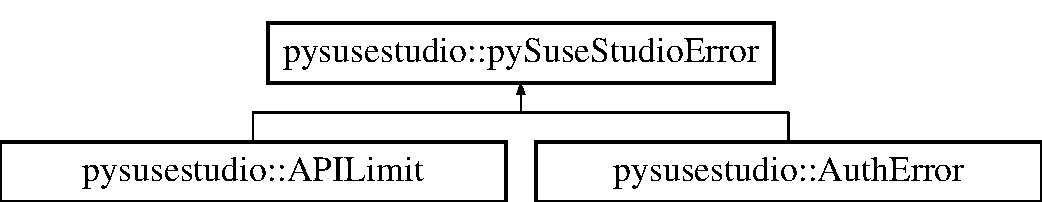
\includegraphics[height=2cm]{classpysusestudio_1_1py_suse_studio_error}
\end{center}
\end{figure}
\subsection*{Public Member Functions}
\begin{DoxyCompactItemize}
\item 
\hypertarget{classpysusestudio_1_1py_suse_studio_error_a33c11152c3ff0ca6d729b89d36eba82c}{
def {\bfseries \_\-\_\-init\_\-\_\-}}
\label{classpysusestudio_1_1py_suse_studio_error_a33c11152c3ff0ca6d729b89d36eba82c}

\item 
\hypertarget{classpysusestudio_1_1py_suse_studio_error_ae5f1e697e1a50f637188a465447e4796}{
def {\bfseries \_\-\_\-str\_\-\_\-}}
\label{classpysusestudio_1_1py_suse_studio_error_ae5f1e697e1a50f637188a465447e4796}

\end{DoxyCompactItemize}
\subsection*{Public Attributes}
\begin{DoxyCompactItemize}
\item 
\hypertarget{classpysusestudio_1_1py_suse_studio_error_abf28bfaa1aa3afdb3b7c4d653e408f23}{
{\bfseries msg}}
\label{classpysusestudio_1_1py_suse_studio_error_abf28bfaa1aa3afdb3b7c4d653e408f23}

\end{DoxyCompactItemize}


The documentation for this class was generated from the following file:\begin{DoxyCompactItemize}
\item 
pysusestudio.py\end{DoxyCompactItemize}

\printindex
\end{document}
